\begin{figure}[htbp]
\section*{SMARCB1}
\centering
\begin{subfigure}[b]{0.75\textwidth}
\centering
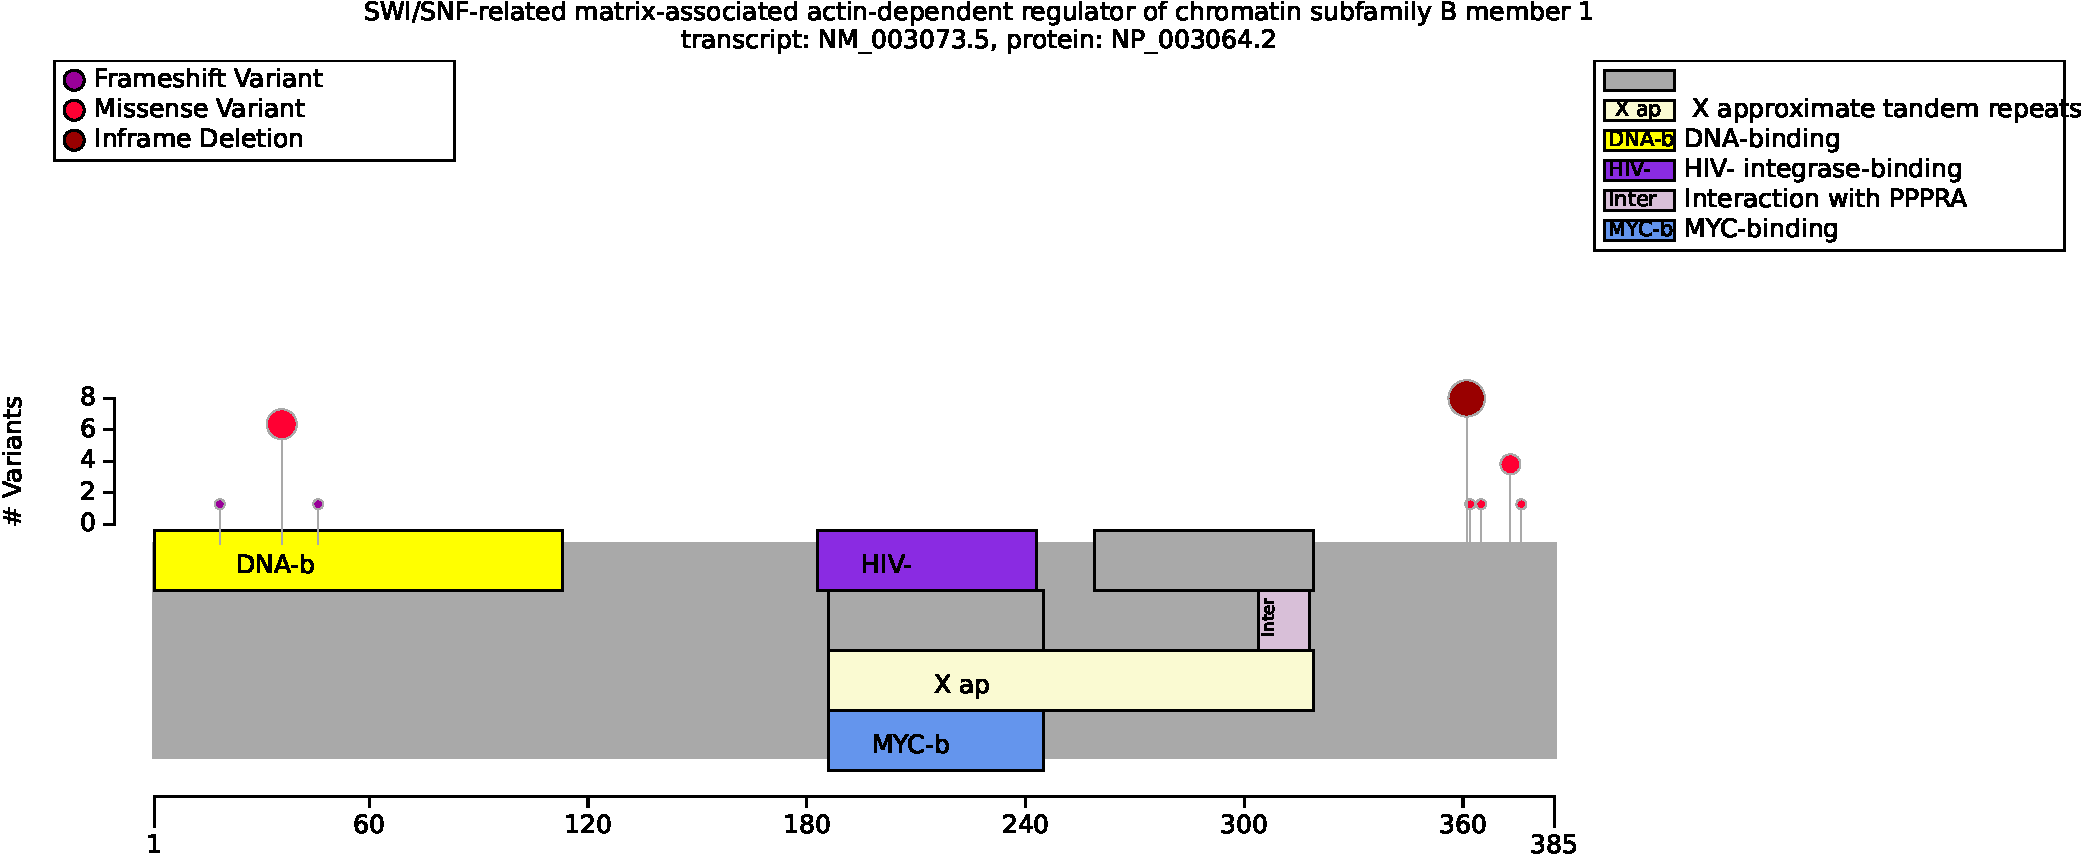
\includegraphics[width=\textwidth]{ img/SMARCB1_protein_diagram.pdf} 
\captionsetup{justification=raggedright,singlelinecheck=false}
\caption{Distribution of variants in SMARCB1}
\end{subfigure}

\begin{subfigure}[b]{0.95\textwidth}
\centering
\resizebox{\textwidth}{!}{
\begin{tabular}{llllrr}
\toprule
HPO term & Structural variant & Other & p-value & adj. p-value\\
\midrule
Atypical teratoid/rhabdoid tumor [HP:0034401] & 8/9 (89\%) & 2/19 (11\%) & $1.19\times 10^{-4}$ & $5.94\times 10^{-4}$\\
Embryonal neoplasm [HP:0002898] & 8/8 (100\%) & 2/19 (11\%) & $2.03\times 10^{-5}$ & $1.52\times 10^{-4}$\\
Neoplasm by histology [HP:0011792] & 11/11 (100\%) & 4/21 (19\%) & $1.06\times 10^{-5}$ & $1.52\times 10^{-4}$\\
Rhabdoid tumor [HP:0034557] & 4/4 (100\%) & 2/19 (11\%) & 0.002 & 0.006\\
Neoplasm by anatomical site [HP:0011793] & 3/3 (100\%) & 3/20 (15\%) & 0.011 & 0.028\\
Neuroepithelial neoplasm [HP:0030063] & 2/2 (100\%) & 0/17 (0\%) & 0.006 & 0.018\\
\bottomrule
\end{tabular}
}
\captionsetup{justification=raggedright,singlelinecheck=false}
\caption{Fisher Exact Test. Total of 15 tests were performed. }
\end{subfigure}
\vspace{1em}
\begin{subfigure}[b]{0.75\textwidth}
\centering
\resizebox{\textwidth}{!}{
\begin{tabular}{llllrr}
\toprule
Genotype (A) & Genotype (B) & total tests performed & significant results\\
\midrule
Lys364del & Other & 52 & 0\\
DNA binding & Other & 51 & 0\\
\bottomrule
\end{tabular}
}
\captionsetup{justification=raggedright,singlelinecheck=false}
\caption{Fisher Exact Test performed to compare HPO annotation frequency with respect to genotypes. }
\end{subfigure}

\caption{The cohort comprised 32 individuals (12 females, 8 males, 12 with unknown sex). 9 of these individuals were 
reported to be deceased. A total of 110 HPO terms were used to annotate the cohort. Disease diagnoses: 
Coffin-Siris syndrome 3 (OMIM:614608) (18 individuals), Rhabdoid tumor predisposition syndrome 1 (OMIM:609322) 
(14 individuals). Our analysis of SMARCB1 included variants associated with Coffin-Siris syndrome 3 (OMIM:614608).
A total of 11 unique variant alleles were found in \textit{SMARCB1} (transcript: \texttt{NM\_003073.5}, 
protein id: \texttt{NP\_003064.2}). Presumably the result of embryonal neoplasm being signficantly associated with structural variants relates to a 
different distribution of variants in rhabdoid tumor predisposition syndrome-1 than in Coffin-Siris syndrome 3.
A published analysis of GPCs in Coffin-Siris syndrome did not present a statistical analysis and did not note the current association \cite{PMID_25168959}.}
\end{figure}

